\subsubsection{方程组}\label{subsec:systems-riemann-problems}

本节陈述一组能够求解方程组 Riemann 问题的结果, 但其中一些证明只针对 $p$ 方程组这个特殊情形. 这样, 既能使论述相当简短而具体, 又能展示更一般证明中涉及的大部分思想.

对单个守恒律, 可以用单个波, 即激波或稀疏波, 连接任意一对左状态与右状态. 在更高维情形下, 必须使用中间状态和几个不同的波来连接. 不过, 作为第一步, 先考察哪些左状态与右状态可以用单个激波或稀疏波"连接起来".

\paragraph*{激波}

\PDEIndexMark{idx:riemann-shock-curves-introduction}首先考虑用单个激波连接左状态与右状态的可能性. 因此需要问: 给定 $\bm{u}^l$, 哪些状态 $\bm{u}^r$ 满足 Rankine-Hugoniot 条件 \eqref{eq:rankine-hugoniot-jump-condition} 和 Lax 激波条件 \eqref{eq:lax-shock-condition}? 答案是, 从状态空间中的每个点 $\bm{u}^l$ 出发, 存在 $n$ 条\emph{激波曲线}, 描述可由单个激波连接的所有可能的右状态. 更具体地说, 有以下定理.

\begin{Theorem}
\label{thm:shock-curves-existence}
假设 \eqref{eq:conservation-law-system} 为定义在状态空间的区域 $\Omega\subset\mathbb{R}^n$ 上的严格双曲守恒律方程组. 那么对任意 $\bm{u}^l\in\Omega$, 都存在 $n$ 个包含 $0$ 的开区间 $I_k$, 以及定义在 $\epsilon\in I_k$ 上的 $n$ 个单参数状态族 $\hat{\bm{u}}_k(\epsilon)$ 和激波速度 $\hat s_k(\epsilon)$, 使得
\begin{equation}\label{eq:shock-curve-base-state}
\bm{u}_k(0)=\bm{u}^l
\end{equation}
且对 $\epsilon\in I_k$, $\hat{\bm{u}}_k(\epsilon)$ 和 $\hat s(\epsilon)$ 满足 Rankine-Hugoniot 条件
\[
\hat s(\epsilon)[\bm{u}^l-\hat{\bm{u}}_k(\epsilon)]=\bm{f}(\bm{u}^l)-\bm{f}(\hat{\bm{u}}_k(\epsilon)).
\]
此外, 若第 $k$ 个特征场真正非线性, 则可选择参数化, 使得
\begin{equation}\label{eq:shock-curve-initial-tangent}
\hat{\bm{u}}_k'(0)=\bm{r}_k(\bm{u}^l),
\end{equation}

\begin{equation}\label{eq:shock-curve-initial-speed}
\hat s(0)=\lambda_k(\bm{u}^l),
\end{equation}

\begin{equation}\label{eq:shock-curve-initial-speed-derivative}
\hat s'(0)=1/2,
\end{equation}
其中撇号 $'$ 表示对 $\epsilon$ 求导. 而且, 采用这一参数化时, Lax 激波条件成立当且仅当 $\epsilon<0$.
\end{Theorem}

不在一般情形下证明这一定理, 而是对 $p$ 方程组显式计算激波曲线. 为保证严格双曲性与真正非线性, 假设 $p'<0$ 和 $p''>0$. 还可假设 $p$ 定义在整个 $\mathbb{R}$ 上, 或对下文所选状态作适当限制. 因此, 取任意容许的 $\bm{u}^l:=(w^l,v^l)^t$, 并假设 $\hat{\bm{u}}:=(\hat w,\hat v)^t$ 由定理所断言存在的两条激波曲线中的一条连接到 $\bm{u}^l$. 此时 Rankine-Hugoniot 条件化为
\begin{equation}\label{eq:p-system-shock-volume-rh}
s(w^l-\hat w)=-(v^l-\hat v),
\end{equation}

\begin{equation}\label{eq:p-system-shock-velocity-rh}
s(v^l-\hat v)=p(w^l)-p(\hat w).
\end{equation}
从这些方程中消去 $s$, 得到
\begin{equation}\label{eq:p-system-shock-eliminated-speed}
(v^l-\hat v)^2=(\hat w-w^l)(p(w^l)-p(\hat w)).
\end{equation}


由于 $p'<0$, 有两条解曲线, 对 $p$ 定义域内的所有 $\epsilon$ 都有定义.
\begin{equation}\label{eq:p-system-first-shock-curve}
\begin{aligned}
S_1:\quad\hat{\bm{u}}_1(\epsilon)&=\begin{pmatrix}\hat w_1(\epsilon)\\\hat v_1(\epsilon)\end{pmatrix}\\
&:=\begin{pmatrix}\epsilon\\v^l+\operatorname{sgn}(\epsilon-w^l)\sqrt{(\epsilon-w^l)(p(w^l)-p(\epsilon))}\end{pmatrix},
\end{aligned}
\end{equation}

\begin{equation}\label{eq:p-system-second-shock-curve}
\begin{aligned}
S_2:\quad\hat{\bm{u}}_2(\epsilon)&=\begin{pmatrix}\hat w_2(\epsilon)\\\hat v_2(\epsilon)\end{pmatrix}\\
&:=\begin{pmatrix}\epsilon\\v^l-\operatorname{sgn}(\epsilon-w^l)\sqrt{(\epsilon-w^l)(p(w^l)-p(\epsilon))}\end{pmatrix}.
\end{aligned}
\end{equation}
相应的激波速度为
\begin{equation}\label{eq:p-system-first-shock-curve-speed}
\hat s_1(\epsilon):=-\sqrt{\dfrac{p(w^l)-p(\epsilon)}{\epsilon-w^l}},
\end{equation}

\begin{equation}\label{eq:p-system-second-shock-curve-speed}
\hat s_2(\epsilon):=\sqrt{\dfrac{p(w^l)-p(\epsilon)}{\epsilon-w^l}}.
\end{equation}


\begin{figure}[H]
\centering
\includegraphics[page=98,pagebox=cropbox,trim=49.99bp 487.10bp 20.59bp 51.92bp,clip,width=.78\linewidth]{../input/source/An Introduction to Partial Differential Equations.pdf}
\caption{}\label{fig:p-system-shock-curves}
\end{figure}

每条曲线仅有一半满足 Lax 激波条件. 条件 \eqref{eq:p-system-back-shock-volume-jump} 和 \eqref{eq:p-system-front-shock-volume-jump} 表明, 1-shock 的任意右状态都必须位于曲线
\begin{equation}\label{eq:p-system-admissible-first-shock-states}
\bm{u}^r=\hat{\bm{u}}_1(\epsilon),\quad\epsilon<w^l,
\end{equation}
上, 而 2-shock 的任意右状态都必须位于曲线
\begin{equation}\label{eq:p-system-admissible-second-shock-states}
\bm{u}^r=\hat{\bm{u}}_2(\epsilon),\quad w^l<\epsilon.
\end{equation}
上. 要求读者验证, 可以重新参数化这些曲线, 使其满足所述初始条件; 更重要的是, 这些状态和对应的激波速度满足 \eqref{eq:p-system-back-shock-speeds} 和 \eqref{eq:p-system-front-shock-speeds} (参见 Problem~\ref{ex:p-system-shock-reparametrization}).

从图上可见, 每个左状态 $\bm{u}^l$ 都发出两条激波曲线 $S_1$ 和 $S_2$. 负速度的激波 (有时称为慢激波或后向激波) 位于 $S_1$ 上; 正速度的激波 (快激波或前向激波) 位于 $S_2$ 上.
